\section{Visual Servoing}
\subsection{Basic Framework of Visual Servoing}
Visual Servoing refers to the family of closed loop control techniques to control the degrees of freedom of an actuated system with visual feedback\cite{chaumette2006visual}. The vision data may be acquired from a camera that is mounted directly on a robot manipulator or on a mobile robot, or the camera can be fixed in the workspace so that it can observe the robot motion from a stationary configuration. Visual Servoing relies on techniques from image processing, computer vision, and control theory.

\begin{figure}[ht!]
  \centering
  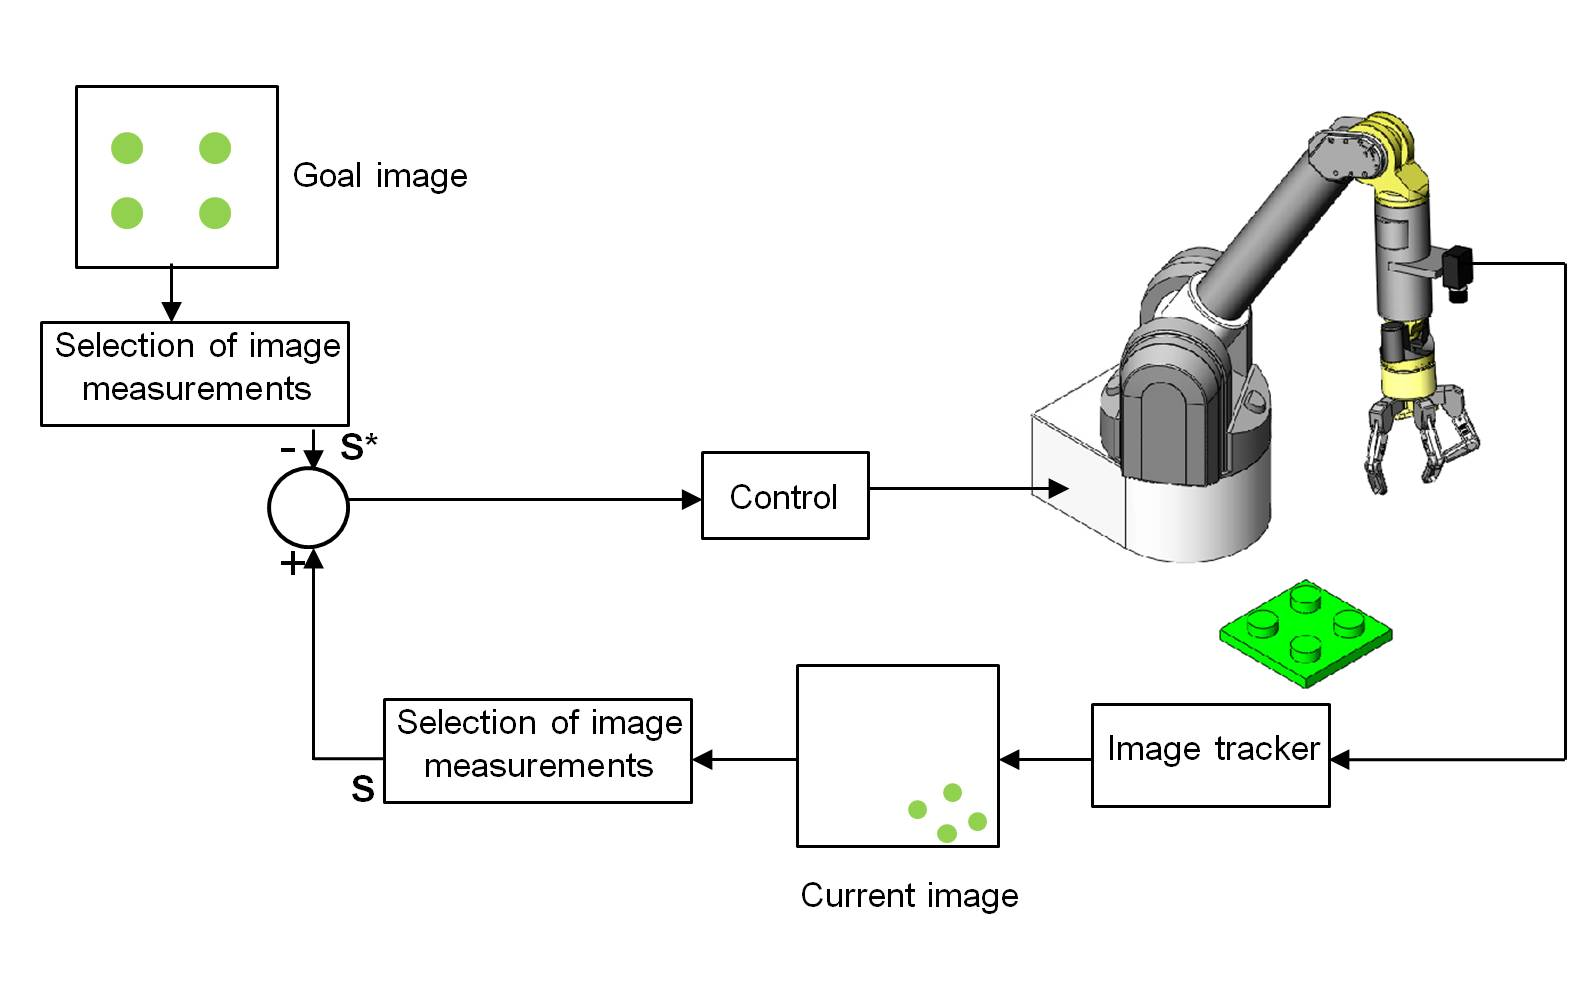
\includegraphics[width=100mm]{figures/vsloop.png}
  \caption{Block diagram of the basic Visual Servoing loop control}
  \label{fig:vsloop}
\end{figure}

The goal of many robotic applications is to place the robot at a desired configuration to manipulate an object in the environment. The objective of closed loop control techniques is to minimize an error $e(t)$ defined as
\begin{equation}
  e(t) = s(t) - s^{*}
  \label{eq:servo1}
\end{equation}
where $s$ is a vector of visual features, and the vector $s^*$ has the desired values of these features at the desired configuration.

Computer vision algorithms are used for the tracking of visual features on the object. There are three main classes of visual servoing: Image-based Visual Servoing (IBVS), Position-based Visual Servoing (PBVS), and Hybrid Visual Servoing (HVS) \cite{chaumette2006visual}\cite{chaumette2007visual}. In IBVS, the features are computed from the 2D image data, while in PBVS, the features are computed from the 3D estimated pose from image measurements. HVS use a combination of 2D and 3D visual features.

Then, to design the control scheme, the relationship between the time variation of the features $s$ and the camera velocity has to be found. Noting the spatial velocity of the camera $u_c = (v_c, \omega_c)$, where $v_c$ is the instantaneous linear velocity of the origin of the camera frame, and $\omega_c$ is the instantaneous angular velocity of the camera frame. The relationship between $\dot{s}$ and $u_c$ is given by
\begin{equation}
  \dot{s} = L_s u_c
  \label{eq:servo2}
\end{equation}

where $L_s$ is called the \textbf{interaction matrix} related to $s$. This matrix relates the rate of changes of the image feature velocities $\dot{s}$ to the rate of change of the pose parameters which is the camera velocity. From~\ref{eq:servo1} and~\ref{eq:servo2}, the relationship between the camera velocity and the derivative of the error is
\begin{equation}
  \dot{e} = L_s u_c
\label{eq:servo3}
\end{equation}

Considering $u_c$ as the input to the robot controller, to ensure an exponential decoupled decrease of the error, we would like to have $\dot{e} = -\lambda e$, using~\ref{eq:servo3} we obtain the control law equation
\begin{equation}
  u_c = -\lambda L_{s}^{+} e
\label{eq:servo4}
\end{equation}
where $L_{s}^{+}$ is the pseudo-inverse of $L_s$. This is the basic visual servoing closed loop system framework. Different visual servoing approaches differ only in the selection of the visual features $s$ and deriving their corresponding interaction matrices $L_s$.

The choice of the visual features is important and generally affect the performance of the visual servoing system.

\subsection{Image-Based Visual Servoing (IBVS)}
In the IBVS approach, the visual features are defined directly in the 2D image space. This is done without the explicit calculation of the relative camera frames at current and desired configurations.

 Considering a 3D point $[X Y Z]^{T}$ expressed in the camera frame and its projection onto the image plane $[x y]^{T}$. If we take the image coordinates in the image plane of the 3D point as visual features, then the corresponding interaction matrix $L_s$ has the following form
 \begin{equation}
L_s = \begin{bmatrix}
  -\frac{1}{Z} & 0 & \frac{x}{Z} & xy & -(1+x^2) & y\\
  0 & -\frac{1}{Z} & \frac{y}{Z} & 1+y^2 & -xy & -x
\end{bmatrix}
\label{eq:servo5}
 \end{equation}
 The value $Z$ is the depth of the point relative to the camera frame. Therefore, any control scheme that uses this form of the interaction matrix must estimate or approximate the value of $Z$. Similarly, the camera intrinsic parameters are involved in the computation of $x$ and $y$. Thus $L_{s}^{+}$ cannot be directly used and an estimation or an approximation $\widehat{L}_s^{+}$ must be used in practice.

The IBVS approach is more robust to modeling and measurement noise than PBVS. However, the IBVS approach only guarantees local asymptotic stability with a local control law theoretically. It also suffers from degenerate cases and fails to reach the goal state.

\subsection{Position-Based Visual Servoing (PBVS)}
In PBVS, the visual features are expressed in terms of the 3D rigid-body transformation from the initial to the desired states, with respect to some reference coordinate frame. The camera acts as a 3D sensor.

First we define three coordinate frame: the current camera frame $F_c$, the desired camera frame $F_{c^*}$ and a reference frame $F_o$ attached to the object. The standard notation is to use a leading superscript to denote the frame with respect to which a set of coordinates is defined.

$s$ can be defined to be $(t,\theta u)$, where $t$ is a translation vector, and $\theta u$ is the angle parameterization for the rotation. If $t$ is defined relative to the object frame $F_o$, then
\begin{equation}
s = (^{c}t_o,\theta u), s^* = (^{c^*}t_o, 0), e = (^{c}t_o - ^{c^*}t_o, \theta u)
\label{eq:servo6}
\end{equation}

And the corresponding interaction matrix is given by
\begin{equation}
  Ls = \begin{bmatrix}
    -\bf{I}_3 & {[^{c}t_o]}_{\times}\\
    \bf{0} & L_{\theta u}
  \end{bmatrix}
\label{eq:servo7}
\end{equation}
where $I_3$ is the $3 \times 3$ identity matrix and $L_{\theta u}$ is given by
\begin{equation}
  L_{\theta u} = I_3 - \frac{\theta}{2}{[u]}_{\times} + \begin{pmatrix} 1 - \frac{sinc \theta}{sinc^2 \frac{\theta}{2}}\end{pmatrix}{[u]}_{\times}^{2}
\label{eq:servo8}
\end{equation}

If the pose parameters are perfectly estimated, the choice of $e$ causes the rotational motion to follow a geodesic with an exponential decreasing speed and causes the translational parameters involved in $s$ to decrease with the same speed. The trajectory in the image of the origin of the object frame follows a pure straight line. However, the camera trajectory does not follow a straight line.

Another PBVS scheme can be designed by choosing $s = (^{c^*}t_c,\theta u)$, which lead to having $s^* = \bf{0}, e = s$, and the following interaction matrix
\begin{equation}
  L_s = \begin{bmatrix}
    R & \bf{0}\\
    \bf{0} & L_{\theta u}
  \end{bmatrix}
\label{eq:servo9}
\end{equation}
This definition introduces a decoupling between translational and rotational motions, which allow a simpler control scheme. The resulting camera trajectory is then a pure straight line.

PBVS approach ensure global asymptotic stability if the pose estimation or tracking is perfect. The pose estimation algorithm must be realized in real-time to calculate the error at every control iteration, and hence more computationally expensive than IBVS approach. However, PBVS approach is more sensitive to image measurement noise and outliers. It also requires full knowledge of the geometric object model, the camera intrinsic calibration, and the robot kinematic calibration.
